\begin{enumerate}[label=\thesubsection.\arabic*,ref=\thesubsection.\theenumi,itemsep=1pt]
 \item In an AP, if $d=2, n=5$ and $a_n=0$, then value of $a$ is
    \hfill (10,  2011)
\begin{multicols}{4}
    \begin{enumerate}
         \item 10
         \item 5
         \item -8
         \item 8
    \end{enumerate}
\end{multicols}
 \item Find whether -150 is a term of the AP: $17, 12, 7, 2,\dots$?
    \hfill (10,  2011) \item Find the value of the middle term of the following AP: $- 6, -2, 2,\dots, 58.$
   \hfill (10,  2011) \item Determine the AP whose fourth term is 18 and the difference of the ninth term from the fifteenth term is 30.
\hfill (10,  2011) \item Find how many two-digit numbers are divisible by $6$.
 How many multiples of $4$ lie between $10$ and $250$ ? Also find their sum.
    \hfill (10,  2011)
         \item The ratio of the $11\textsuperscript{th}$ term to $17\textsuperscript{th}$ term of an AP is $3:4$. Find the ratio of $5\textsuperscript{th}$ to $21\textsuperscript{th}$ of the same AP. Also, find the ratio of the sum of first $5$ terms to that of first $21$ terms
        \hfill (10,  2023) \item $250$ logs are stacked in the following manner:
        $22$ logs in the bottom row, $21$ in the next row, $20$ in the row next to it and so on. In how many rows are the $250$ logs placed and how many logs are there in top row ?
\hfill (10,  2023)
 \item If $-\frac{5}{7}$, $a$, $2$ are consecutive terms in an Arthimetic Progression, then the value of $a$ is 
    \hfill (10,  2022)
    \begin{multicols}{4}
\begin{enumerate}    
\item $\frac{9}{7}$
 \item $\frac{9}{14}$
 \item $\frac{19}{7}$
 \item $\frac{19}{14}$
    \end{enumerate}
\end{multicols}
 \item Find the sum of first $16$ terms of an Arithmetic Progression whose $4^{\text{th}}$ and $9^{\text{th}}$ terms are $-15$ and $-30$ respectively.
        \hfill (10,  2022) \item If the sum of first $14$ terms of an Arithmetic Progression is $1050$ and its fourth term is $40$, find its $20^{\text{th}}$ term.
\hfill (10,  2022)
         \item Find the sum of the first twelve $2$-digit numbers which are 
multiples of $6$.
\hfill (10,  2022)
         \item In an AP, if $a_2=26$ and $a_{15} = -26$, then write the AP.
\hfill (10,  2022)
         \item In Mathematics, relations can be expressed in various ways. The 
matchstick patterns are based on linear relations. Different strategies 
can be used to calculate the number of matchsticks used in different 
		\figref{fig:ap} 
One such pattern is shown below. Observe the pattern and answer the 
following questions using Arithmetic Progression 

    \hfill (10,  2022) 
\begin{figure}[H]
    \centering
	\includegraphics[width=\columnwidth]{figs/ap/ap.jpg}
	\caption{}
    \label{fig:ap}
\end{figure}
    \begin{enumerate}
	 \item Write the AP for the number of triangles used in the \figref{fig:ap}. Also, 
write the nth term of this AP.
 \item Which figure has $61$ matchsticks ? 
    \end{enumerate} 
 \item In an AP if the sum of third and seventh term is zero, find its $5^{\text{th}}$ term.
        \hfill (10,  2022)
  \item Determine the AP whose third term is $5$ and seventh term is $9$.
        \hfill (10,  2022) \item Find the sum of the first $20$ terms of an AP whose $n^{\text{th}}$ term is given as $a_n=5-2n$

%
        \hfill (10,  2022) \item Find the common difference $d$ of an AP whose first term is $10$ and the sum of the first $14$ terms is $1505$.
        \hfill (10,  2022) \item For what value of $n$, are the $n^{\text{th}}$ terms of the APs: $9,7,5,\dots$ and $15,12,9,\dots$ the same?
    \hfill (10,  2022)
	 \item Write the common difference of the AP: $\frac{1}{5}, \frac{4}{5}, \frac{7}{5}, \frac{10}{5}, \cdots$
	\hfill (10,  2021) \item Find the $8^{th}$ term of the AP whose first term is $-2$ and common difference is $3$.

%
	\hfill (10, 2021) \item
	Roshini being a plant lover decides to start a nursery. She bought few plants with pots. She placed the pots in such a way that the number of pots in the first row is $2$, in the second is $5$, in the third row is $8$ and so on as shown in 
			\figref{fig:Plants}.
		\begin{figure}[H]
			\centering	
			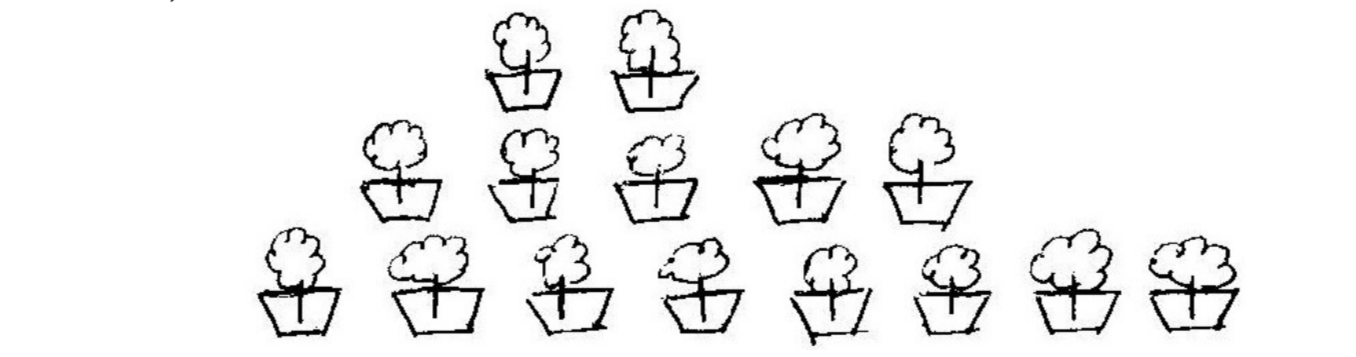
\includegraphics[width=\columnwidth]{figs/ap/Plant.png}
			\caption{}
			\label{fig:Plants}
		\end{figure}
		Based on the above, answer the following questions 
\hfill (10, 2021)
		\begin{enumerate}
\item How many pots were placed in the $7^{th}$ row ?
				\begin{multicols}{4}
\begin{enumerate}    
					 \item $20$
					 \item $23$
					 \item $77$
					 \item $29$
				\end{enumerate}
\end{multicols}
 \item If Roshini wants to place $100$ pots in total, then total number of rows formed in the arrangement will be ?
				\begin{multicols}{4}
\begin{enumerate}    
					 \item $8$
					 \item $9$
					 \item $10$
					 \item $12$
				\end{enumerate}
\end{multicols}
 \item How many pots are placed in the last row ?
				\begin{multicols}{4}
\begin{enumerate}    
					 \item $20$
					 \item $23$
					 \item $26$
					 \item $29$
				\end{enumerate}
\end{multicols}
			 \item If Roshini has sufficient space for $12$ rows, then how many total number of pots are placed by her wih the same arrangement ?
				\begin{multicols}{4}
\begin{enumerate}    
					 \item $222$
					 \item $155$
					 \item $187$
					 \item $313$
				\end{enumerate}
\end{multicols}
		\end{enumerate} 
	 \item The sum of the first $4$ terms of an AP is zero and its $4^{th}$ term is $2$. Find the AP.

	\hfill (10, 2021) \item If the sum of the first $n$ terms of an AP is given by $S_n = 4n - n^2$, then find its $n^{th}$ term. Hence, find the $25^{th}$ term and the sum if the first 25 terms of this AP.

\hfill (10, 2021)
	 \item Find the mean of first $10$ composite numbers.
	\hfill (10, 2021) \item If $S_n$ denotes the sum of first $n$ terms of an AP, prove that $S_{12} = 3(S_8 - S_4)$.

%
	\hfill (10, 2021) \item After how many decimal places will the decimal expansion of the rational number $\frac{14587}{1250}$ terminate ?			
\hfill (10, 2021)
	 \item If the $6^{th}$ and $14^{th}$ terms of an AP are 29 and 69 respectively, then find the $10^{th}$ term of the AP.
	\hfill (10, 2021) \item If the first three consecutive terms of an AP are $3y-1, 3y+5$ and $5y+1$ find the value of $y$. 
\hfill (10, 2021)
 \item Which of the following is not an AP? 
\hfill (10, 2020)
\begin{multicols}{2}
\begin{enumerate}    
               \item $-1.2,0.8,2.8,\dots$ 
	        \item $3,3+\sqrt2,3+2\sqrt2,3+3\sqrt2,\dots$ 
	        \item $\frac{4}{3},\frac{7}{3},\frac{9}{3},\frac{12}{3},\dots$ 
	        \item $\frac{-1}{5},\frac{-2}{5},\frac{-3}{5},\dots$ 
\end{enumerate}
\end{multicols}
 \item Find the sum of the first $100$ natural numbers.	
	\hfill (10, 2020)
 \item Find the sum
\hfill (10, 2020)
\begin{align*}
	\brak{-5} + \brak{-8} + \brak{-11} + \dots + \brak{-230}
\end{align*}
 \item Find the number of terms in the AP 
    $18,15\frac{1}{2},13, \dots, 47.$
\hfill (10, 2019) \item Determine the AP whose third term is $16$ and $7^{th}$ term exceeds the $5^{th}$ term by $12$.

%
\hfill (10, 2019) \item Find the value of $x$, when in the AP given below
\hfill (10, 2019)
\begin{align*}
2 + 6 + 10 + \dots + x = 1800.    
\end{align*}
 \item Which term of the AP $-4, - 1, 2, \dots$ is $ 101$?
\hfill (10, 2019) \item In an AP, the first term is $- 4$, the last term is $29$ and the sum of all its terms is $150$. Find its common difference.
\hfill (10, 2019) \item Find the $21^{st}$ term of the AP $-4 \frac{1}{2},-3,-1\frac{1}{2}, \dots $
\hfill (10, 2019) \item Find the common difference of the AP 
\hfill (10, 2019)
\begin{align*}
\frac{1}{a} , \frac{3-a}{3a},\frac{3-2a}{3a} , \dots (a \neq 0)
\end{align*}
 \item Which term of the Arithmetic Progression $-7, -12, -17, -22, \dots$ will be $-82$? Is $-100$ any term of the AP? Give reason for your answer.
\hfill (10, 2019) \item How many terms of the Arithmetic Progression $45, 39, 33,  \dots  $ must be taken so that their sum is $180$ ? Explain the double answer.
\hfill (10, 2019) \item Find after how many places of decimal the decimal form of the number $\frac {27}{2^35^43^2}$ will terminate.
\hfill (10, 2019) \item Find the sum of first $10$ multiples of $6$

\hfill (10, 2019) \item If $m$ times the $m^{th}$ term of an Arithmetic Progression is equal to $n$ times
its $n^{th}$ term and $m \neq n$, show that the $\brak{m + n}^{th}$ term of the A.P is zero
\hfill (10, 2019) \item The sum of the first three numbers in an Arithmetic Progression is $18$. If the product of the first and the third term is $5$ times the common
difference, find the three numbers.
 \item Find the sum of all the two digit numbers which leave the remainder $2$ when divided by $5$.
\hfill (10, 2019) \item If in an AP, $a=15$, $d=-3$ and $a_n=0$, then find the value of $n$.
\hfill (10, 2019) \item If ${S_n}$, the sum of the first ${n}$ terms of an AP is given by ${S_n = 2n^2 + n}$, then find its $n^{th}$ term. 
\hfill (10, 2019) \item If the $17^{th}$ term of an AP exceeds its $10^{th}$ term by $7$, find the common difference.

\hfill (10, 2019) \item If the sum of the first $p$ terms of an AP is $q$ and the sum of the first $q$ terms is $p$, then show that the sum of the first $\brak{p + q}$ terms is $\cbrak {-\brak {p + q}}$.
%
\hfill (10, 2019) \item Write the common difference of the AP${\sqrt3} , {\sqrt12} , {\sqrt27} , {\sqrt48}$ ,  \dots  
%
\hfill (10, 2019) \item In an AP, the $n^{th}$ term is ${\frac{1}{m}}$ and the $m^{th}$ term is $\frac{1}{n}$. Find 
\hfill (10, 2019)
\begin{enumerate}
      \item  $\brak{mn}^{th}$ term,
      \item sum of first $\brak{mn}$ terms.
\end{enumerate}
%
 \item The first term of an AP is 3, the last term is 83 and the sum of all its terms is 903. Find the number of terms and the common difference of the AP.
 \hfill (10, 2019) \item If the sum of first $n$ terms of an  AP  is $n^2$, then find its $10^{th} $term.
\hfill (10, 2019) \item Which term of the AP: $3, 15, 27, 39, \dots$ will be $120$ more than its $21$st term?

\hfill (10, 2019) \item If $S_n$, the sum of first $n$ terms of an  AP  is given by $S_n=3n^2-4n$, find the $n^{th}$ term.

\hfill (10, 2019) \item If the sum of first four terms of an  AP  is $40$ and that of first $14$ terms is $280$. Find the sum of its first $n$ terms.
\hfill (10, 2019)
%
			 \item In an  AP , if the common difference $d = -4$, and the seventh term $a_7$ is $4$, then find the first term.		
			\hfill (10, 2018) \item The sum of four consecuive numbers in an AP is $32$ and the ratio of the product of the first and the last term to the product of two middle term is $7:15$. Find the numbers.
	\hfill (10, 2018) \item Find the sum of $8$ multiples of $3$.
\hfill (10, 2018)
%
			 \item In an  AP , if the common difference $d = -4$, and the seventh term $a_7$ is $4$, then find the first term.		
			\hfill (10, 2018) \item The sum of four consecuive numbers in an AP is $32$ and the ratio of the product of the first and the last term to the product of two middle term is $7:15$. Find the numbers.
%
	\hfill (10, 2018) \item Find the sum of $8$ multiples of $3$.
\hfill (10, 2018)
 \item The $5^{th}$ and $15^{th}$ terms of an AP are $13$ and $-17$ respectively. Find the sum of first $21$ terms of the AP.
\hfill (10, 2018)
%
 \item The sum of the first $n$ terms of an AP is $5n^{2}+3n$. If its $m^{th}$ terms is $168$, find the value of $m$. Also find the $20^{th}$ term of the AP.
\hfill (10, 2018) \item The $4^{th}$ and the last terms of an AP are $11$ and $89$ respectively. If there are $30$ terms in the AP, find the A.P and its $23^{rd}$ term.
\hfill (10, 2018) \item Write the $m^{th}$ term of the AP $$\frac{1}{k},\dfrac{1+k}{k},\dfrac{1+2k}{k},\dots$$
\hfill (10, 2018)
 \item Which term of the AP: $8,14,20,26,\dots$ will be $72$ more than its $41^{st}$ term ?

\hfill (10, 2017) \item If the $10^{th}$ term of an AP is $52$ and the $17^{th}$ term is $20$ more than the $13^{th}$ term, find the AP
\hfill (10, 2017) \item If the ratio of the sum of the first n terms of two A.Ps is $\brak{7n + 1}$ : $\brak{4n + 27}$, then find the ratio of their $9^{th}$ terms.
\hfill (10, 2017) \item For what value of $n$, are the $n^{th}$ terms of two APs $63,65,67,\dots$ and $3,10, 17,\dots$ equal?
\hfill (10, 2017) \item How many terms of an AP: $9,17,254,\dots$ must be taken to  give a sum of $636$?

\hfill (10, 2017) \item What is the common difference of an A.P in which $a_{21} - a_7 = 84$ ?
\hfill (10, 2017) \item Which term of the progression $20,19\frac{1}{4},18\frac{1}{2},17\frac{3}{4},\dots$ is the first negative term ?

\hfill (10, 2017) \item The first term of an AP is $5$, the last term is $45$ and the sum of all its terms is $400$. Find the number of terms and the common difference of the AP.
\hfill (10, 2017)
 \item For what value of $k$ will $k+9, 2k-1$ and $2k+7$ are the consecutive terms of an AP ?
 \hfill (10, 2016) \item  The $4^{th}$ term of an AP is zero. Prove that the $25^{th}$ term of the AP is three times its $11^{th}$ term.
 \hfill (10, 2016) \item  If the ratio of the sum of first $n$ terms of two APs is $\brak{7n + 1} : \brak{4n + 27}$, find the ratio of their $m^{th}$ terms.
\hfill (10, 2016) \item The sums of first $n$ terms of three arithmetic progressions are $S_1, S_2$ and $S_3$ respectively. The first term of each AP is $1$ and their common differences are $1, 2$ and $3$ respectively. Prove that $S_1+S_3=S_2$.

\hfill (10, 2016) \item The digits of a positive number of three digits are in AP and their sum is $15$. The number obtained by reversing the digits is $594$ less than the original number. Find the number.
\hfill (10, 2016) \item The houses in a row are numbered consecutively from $1$ to $49$. Show that there exists a value of $X$ such that sum of numbers of houses preceeding the house numbered $X$ is equal to sum of the numbers of houses following $X$.
\hfill (10, 2016)
 \item In an AP, if $S_5 + S_7$ = $167$ and $S_10$ = $235$, then find the AP, where $S_n$ denotes the sum of its first n terms.
\hfill (10, 2015) \item The $14^{th}$ term of an AP is twice its $8^{th}$ term. If its $6^{th}$ term is – $8$, then find the sum of its first $20$ terms.
\hfill (10, 2015) \item Find the $60^{th}$ term of the AP $8, 10,  12,  \dots ,$ if it has a total of 60 terms and hence find the sum of its last $10$ terms.
\hfill (10, 2015) \item The $16^{th}$ term of an {AP} is five times its third term. If its $10^{th}$ term is $41$, then find the sum of its first fifteen terms.
\hfill (10, 2015)
 \item An arithmetic progression $5, 12, 19,  \dots $ has $50$ terms. Find its last term. Hence find the sum of its last $15$ terms.
%
\hfill (10, 2015) \item The $13^{th}$ term of an AP is four times its $3^{rd}$ term. If its fifth term is $16$, then find the sum of its first ten terms.
\hfill (10, 2015)
 \item If the $n^{th}$ term of an AP is $\brak{2n+1}$, then sum of its first three terms is 
\hfill (10, 2012)
\begin{multicols}{4}
\begin{enumerate}
 \item $6n + 3$ 
 \item $15$ 
 \item $12$ 
 \item $21$ 
\end{enumerate}
\end{multicols}
 \item The next term of AP: $\sqrt {18}, \sqrt {50}, \sqrt {98}, \dots$ is \hfill (10, 2012)
\begin{multicols}{4}
\begin{enumerate}
 \item $\sqrt {146}$ 
 \item $\sqrt {128}$ 
 \item $\sqrt {162}$ 
 \item $\sqrt {200}$ 
\end{enumerate}
\end{multicols}
%discrete
 \item Find the common difference of an AP whose first term is $5$ and the sum of its first four terms is half the sum of the next four terms. 
%discrete
 \hfill (10, 2012) \item The $17th$ term of an AP is $5$ more than twice its $8^{th}$ term. If the $11th$ term of the AP is $43$, then find the $n^{th}$ term. 
%
\hfill (10, 2012) \item Sum of the first $14$ terms of an  AP  is $1505$ and its first term is $10$. Find its $25^{th}$ term. 
\hfill (10, 2012) \item In an  AP , the first term is $12$ and the common difference is $6$. If the last term of the  AP  is $252$, find its middle term. 
\hfill (10, 2012) \item If $4$ times the fourth term of an  AP  is equal to $18$ times its $18^{th}$ term, then find its $22^{th}$ term. 
\hfill (10, 2012) \item The sum of $4^{th}$ and $8^{th}$ term terms of an  AP  is $24$ and the sum of its $6^{th}$ and $10^{th}$ terms is $44$. Find the sum of first ten terms of the  AP  
\hfill (10, 2012)
\item In an AP, if $d=2, n=5$ and $a_n=0$, then value of $a$ is
    \hfill (10, 2011)
    \begin{multicols}{4}
\begin{enumerate}
%
\item 10
%
\item 5
%
\item -8
%
\item 8
    \end{enumerate}
\end{multicols}
\item Find whether -150 is a term of the AP: $17, 12, 7, 2,\dots$?
    \hfill (10, 2011)
\item Find the value of the middle term of the following AP: $- 6, -2, 2,\dots, 58.$
   \hfill (10, 2011)
\item Determine the AP whose fourth term is 18 and the difference of the ninth term from the fifteenth term is 30.
    \hfill (10, 2011)
\item
	{Assertion ($A$):} $a,b,c$ are in  AP  if and if only if $2b = a + c$.
%
{Reason($R$):} The sum of first $n$ natural numbers is $n^2$.
\hfill (10, 2023)
\begin{enumerate}
\item Both Assertion $\brak{A}$ and Reason $\brak{R}$ are true and Reason $\brak{R}$ is the correct explanation of Assertion $\brak{A}$.
\item Both Assertion $\brak{A}$ and Reason $\brak{R}$ are true and Reason $\brak{R}$ is not the correct explanation of Assertion $\brak{A}$.
\item Assertion $\brak{A}$ is true but Reason $\brak{R}$ is false.
\item Assertion $\brak{A}$ is false but Reason $\brak{R}$ is true.
\end{enumerate}
\item
How many terms are there in  AP  whsoe first and fifth term are $-14$ and $2$, respectively and the last term is $62$.
\hfill (10, 2023)
\item
Which term of the AP: $65,61,57,53, \dots$ is the first negative term?
\hfill (10, 2023)
\item Three bells ring at intervals of  6, 12 and 18 minutes. If all the three bells rang at  6 a.m., when will they ring together again ?
\hfill (10, 2023)
\item For what value of $k$ will $(k+9), (2k-1)$ and $( 2k+7)$ be consecutive terms of an AP?

\hfill (10, 2016)
\item The sums of the first $n$ terms of three arithmetic progressions are $S_0, S_2$ and $S_3$ respectively. The first term of each AP is $1$ and their common differences are $1, 2$ and $3$ respectively. Prove that $S_1 + S_3 = 2S_2$.
								\hfill (10, 2016)
\item The $5^{\text{th}}$ term of an Arithmetic Progression (AP) is 26 and the 10th term is 51. Determine the $15^{\text{th}}$ term of the AP.
    \hfill (10, 2006)
\item Find the sum of all the natural numbers less than 100 which are divisible by 6.

    \hfill (10, 2006)
\item Find how many two-digit numbers are divisible by $6$.
    \hfill (10, 2011)
\item  How many multiples of $4$ lie between $10$ and $250$ ? Also find their sum.
    \hfill (10, 2011)
\item The sum of first 20 odd natural numbers is : 
    \hfill (10, 2012)
    \begin{multicols}{4}
\begin{enumerate}
\item $100$ 
\item $210$ 
\item $400$ 
\item $420$ 
\end{enumerate}
\end{multicols}
\item How many two-digit numbers are divisible by 3? 
    \hfill (10, 2012)
\item Find the sum of all multiples of 7 lying between $500$ and $900$. 
    \hfill (10, 2012)
\item Find the sum of all three digit natural numbers, which are multiples of $11$. 
    \hfill (10, 2012)
\item Find the sum of first 40 positive integers divisible by $6$. 
    \hfill (10, 2012)
\item How many multiples of $4$ lie between $10$ and $205$?   
    \hfill (10, 2019)
\item Find the number of terms in the following AP
 \hfill (10, 2022) 
            \begin{align*}
                5,11,17,\dots,203
            \end{align*}
	\item While buying an expensive item like a house or a car, it becomes easier for a middle-class person to take a loan from a bank and then repay the loan along with interest in easy instalments. 
          Aman buys a car by taking a loan of \rupee 2,36,000 from the bank and starts repaying the loan in monthly instalments. He pays \rupee 2,000 as the first instalment and then increases the instalment by \rupee 500 every month. 
\hfill (10, 2022)
        \begin{enumerate}
         \item Find the amount he pays in the $25^{\text{th}}$ installment.
 \item Find the total amount paid by him in the first $25$ installments.
        \end{enumerate}
 \item The sum of the first three terms of an AP is $33$. If the product of first and third term exceeds the second term by $29$, find the AP.
         \hfill (10, 2022)    
 \item If $p-1$, $p+1$ and $2p+3$ are in AP, then the value of $p$ is
        \hfill (10, 2023)
        \begin{enumerate}
		\begin{multicols}{4}
       \item $-2$
       \item $4$
       \item $0$
       \item $2$
		\end{multicols}
      \end{enumerate}
    \hfill (10, 2023) 
\item The next term of the AP: $\sqrt{7}, \sqrt{28}, \sqrt{63}$ is 
\hfill (10, 2023)
    \begin{enumerate}
		\begin{multicols}{4}
       \item $\sqrt{70}$
       \item $\sqrt{80}$
       \item $\sqrt{97}$
       \item $\sqrt{112}$
		\end{multicols}
    \end{enumerate}
\item In an A.P., if the first term $a = 7, n^{th}$ term $a_{n} = 84$, and the sum of the first $n$ terms $S_{n} = \frac{2093}{2}$, then $n$ is equal to
\hfill (10, 2024)
\begin{enumerate}
    \item $22$
    \item $24$
    \item $23$
    \item $26$
\end{enumerate}
\item  The sum of first and eighth term of an AP is $32$ and their product is $60$. Find the first term  and common difference of the AP. Hence,also find the sum of its first $20$ terms.
\hfill (10, 2024)
\item In an AP of $40$ terms, the sum of first $9$ terms is $153$ and the sum of last $6$ terms is $687$.
Determine the first term and common difference of AP. Also, find the sum of all the terms of the AP.
\hfill (10, 2024)


\end{enumerate}
%
